\documentclass{scrartcl}
\usepackage[utf8]{inputenc}
\usepackage[frenchb]{babel}
\usepackage{amssymb}
\usepackage{lmodern}
\usepackage[T1]{fontenc}
\usepackage{hyperref}
\usepackage{verbatim}
\usepackage{listings}
\usepackage{graphicx}
\usepackage{amsmath}

\usepackage{color}
\definecolor{deepblue}{rgb}{0,0,0.5}
\definecolor{deepred}{rgb}{0.6,0,0}
\definecolor{deepgreen}{rgb}{0,0.5,0}

\newcommand{\brokencell}[2][c]{\begin{tabular}[#1]{@{}c@{}}#2\end{tabular}}

\lstset{frame=single, breaklines=true,
          breakatwhitespace=true, basicstyle=\scriptsize,
          showstringspaces=false, escapeinside={(*}{*)},
          keywordstyle=\color{deepblue},
          stringstyle=\color{deepred},
          commentstyle=\color{deepgreen},
          literate=
                   {é}{{\'e}}1{É}{{\'E}}1
                   {è}{{\`e}}1{È}{{\`E}}1
                   {ê}{{\^e}}1{Ê}{{\^E}}1
                   {à}{{\`a}}1{À}{{\`A}}1
                   {ù}{{\`u}}1{Ù}{{\`U}}1
                   {û}{{\^u}}1{Û}{{\^U}}1
                   {ô}{{\^o}}1{Ô}{{\^O}}1
                   {ó}{{\'o}}1{Ó}{{\'O}}1
                   {ç}{{\c c}}1{Ç}{{\c C}}1
                   {œ}{{\oe}}1{Œ}{{\OE}}1
        }

\begin{document}
\title{Rapport du projet de programmation stochastique}
\author{Maxence Ahlouche \and Maxime Arthaud \and Korantin Auguste
  \and Martin Carton \and Thomas Forgione \and Thomas Wagner}
\date{27 novembre 2013}
\maketitle
\tableofcontents
\newpage

\section{Présentation de l'équipe}
  Cette équipe a été menée par Thomas Wagner, assisté de son Responsable
  Qualité Korantin Auguste. Les autres membres de l'équipe sont Martin Carton,
  Maxence Ahlouche, Maxime Arthaud, et Thomas Forgione.

  Tous les membres de l'équipe ont été présents à chacune des séances lors de
  cette UA.

\section{Colonie de scarabées}
  Le problème consiste, à partir d'un graphe dont les nœuds représentent des
  positions et les arêtes contiennent la probabilité pour un scarabée de passer
  d'une position à l'autre, à calculer les probabilités de présence de chaque
  scarabée au bout de $N$ itérations, selon sa position de départ.

  Pour cela, on représente le graphe sous la forme de matrice d'adjacence, ou
  chaque élément de la matrice représente la probabilité de passer d'un nœud à
  un autre.

  Si on met cette matrice à la puissance $N$, elle contiendra les probabilités
  de passer d'un nœud à un autre en exactement $N$ itérations.

  En multipliant cette matrice par un vecteur contenant uniquement des zéros,
  sauf au nœud de départ (on mettra un 1), on peut obtenir la probabilité pour
  le scarabée de se trouver à chaque point, au bout d'exactement $N$ tours.  Si
  cette probabilité est nulle, il est impossible qu'il s'y trouve.

  Pour savoir la probabilité que les deux scarabées se rencontrent en un point
  au bout de $N$ itérations, il suffit de multiplier les probabilités de
  présence de chaque scarabée en ce point. Pour connaitre leur probabilité de se
  rencontrer en n'importe quel point, on peut tout simplement sommer les
  probabilités de rencontre sur chaque point.

  De plus, si on calcule $\lim_{N \to \infty} A^N$ (une telle limite n'existera
  que si la chaîne est irréductible, récurrente positive et apériodique, et ça
  ne sera pas toujours le cas!), le produit du vecteur avec la position de
  départ par cette matrice nous donnera les probabilités pour le scarabée
  d'être en chaque position une fois qu'il aura suffisamment voyagé et que sa
  position de départ n'aura plus d'importance.
  %TODO: c'est quoi une chaine irréductible blabla apériodique?

  \subsection{Chaînes de Markov}
    Le problème des scarabées peut aisément être modélisé
    par des chaînes de Markov. En effet, nos coléoptères se promènent en temps
    discret dans leur graphe de promenade; de plus, l'état d'un scarabée
    (autrement dit, sa position dans sa promenade) ne dépend pas du passé, mais
    uniquement de l'état présent.

    La matrice de transition de notre promenade représente les probabilités de
    passer d'un état aux autres. Par conséquent, la matrice de transition à la
    puissance $n$ représente la probabilité de passer d'un état à un autre par
    un chemin de longueur $n$.

    On constate qu'on se rapproche beaucoup de la matrice décrite précédemment : la matrice d'adjacence du graphe de promenade et la
    matrice de transition de notre chaîne de Markov sont équivalentes!

  \subsection{Temps moyen entre rencontre}
    \subsubsection{À partir d'un certain point}
      Considérons que les deux scarabées sont sur le même point.  On peut donc
      calculer la probabilité qu'après $N$ tours, ils finissent à nouveau sur
      la même case (en sommant le carré des probabilités que chacun se retrouve
      sur une case).

      Notons $U_k = pA^k(pA^k)^\intercal$ la probabilité que les deux scarabées
      se retrouvent sur la même case après $k$ tours.

      Notons $V_k$ la probabilité que les deux scarabées se retrouvent sur la
      même case après $k$ tours, sans s'être déjà rencontrés avant. On a:
        \[V_k = (1 - U_1) \times (1 - U_2) \times \cdots \times (1 - U_{k - 1})
        \times U_k\]

      $V_k$ peut donc se réécrire par récurrence:
        \begin{align*}
          V_1       &= U_1 \\
          V_{k + 1} &= V_k \times \frac{1 - U_k}{U_k}U_{k + 1}
        \end{align*}

      Pour avoir le temps moyen au bout duquel ils vont se rencontrer en
      partant de ce même point, il suffit de prendre l'espérance de cette suite
      $V_k$. %TODO: qui est?

    \subsubsection{À partir de deux points différents}
      Dans le cas où les points de départs des scarabées sont différents, on peut
      appliquer le même principe.

      Par contre, on ne peut pas supposer $U_k \neq 0$.
      On peut introduire une suite $W_k$:
      \begin{align*}
        W_0 &= 1 \\
        W_k &= W_{k-1} \times (1 - U_k)
      \end{align*}

      On a donc:
      \begin{align*}
        V_1  &= U_1 \\
        V_k &= W_{k-1} \times U_k
      \end{align*}

      Pour avoir un temps moyen de rencontre global, on fait la moyenne du temps
      de rencontre pour chaque position initiale possible. %TODO: qui est?

\section{Gare de péage}
  Le but de ce problème est de déterminer si une gare de péage constituée de
  plusieurs couloirs de payement est efficace. C'est à dire si le temps
  d'attente ne sera pas trop élevé et si il n'y a aucun couloir ouvert mais
  inutile. Le nombre de voitures qui arrivent par unité de temps et le temps
  mis pour payer (sans compter l'attente) suivent des lois de Poisson.

  Dans la suite, on notera $S$ le nombre de files, $\lambda$ la fréquence à
  laquelle les voitures entrent dans le système et $\mu$ la fréquence moyenne à
  laquelle elles sortent\footnote{C'est à dire $\frac 1 \lambda$ et
  $\frac 1 \mu$ sont respectivement les temps moyens entre deux arrivés et le
  temps moyen que prennent les gens pour payer: $\lambda$ et $\mu$ sont les
  paramètres des lois de Poisson régissant l'entrée et la sortie.}.

  Ce problème donc est celui d'une file d'attente de type $M/M/S$ (où $M/M$
  représente le fait que les lois d'entrés et sorties suivent des lois de
  Poisson).

  \subsection{Analyse}
    On peut montrer que le temps d'attente converge si et seulement si $\psi =
    \frac \lambda {S\mu} < 1$. Il faudra donc ouvrir au moins $\frac \lambda
    \mu$ files.

    De plus, le temps d'attente moyen dans le système étant donné par
      \[T_S = \frac 1 \mu \frac 1 {1-\psi}\]
    pour le limiter à $T_{max}$ temps maximum que l'on veut faire attendre les
    clients il faudra \[\frac {T_{max}\lambda}{\mu T_{max}-1} < S\]

    Or $\frac 1 \mu < \frac{T_{max}}{\mu T_{max}-1}$ (car évidement $T_{max} >
    \frac 1 \mu$), il faudra donc ouvrir au moins
      \[\frac{T_{max}\lambda}{\mu T_{max}-1}\]
    files.

    Si il y plusieurs moyens de payement possibles avec un moyen de payement
    par file, le problème se découpe en plusieurs problèmes indépendants: un
    par type de payement. Il suffit de remplacer ci-dessus $\lambda$ par
    $p_i\lambda$ avec $p_i$ la probabilité qu'une voiture choisisse le moyen de
    payement $i$ et remplacer $\mu$ par $\mu_i$ avec $\frac 1 {\mu_i}$ le temps
    moyen de payement en utilisant le moyen de payement $i$.

    Si il y a des files qui permettent d'utiliser plusieurs moyens de payement
    cependant le problème est plus compliqué.

  \subsection{Simulation sisyphe}
    \subsubsection{Cas d'une file}
      Nous avons commencé par simuler un cas plus simple: celui où il n'y a
      qu'une seule file d'attente.

      \begin{figure}[htbp]
        \centering
        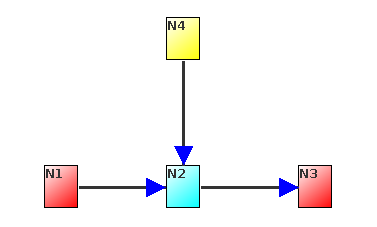
\includegraphics[height=5cm]{img/poisson_simple.png}
        \caption{Modélisation d'une gare de péage avec une seule file}
        \label{figure:syphilis_simple}
      \end{figure}

      Nous avons représenté une file à l'aide de 4 éléments (voir
      figure~\ref{figure:syphilis_simple}):
      \begin{itemize}
        \item l'élément $N1$ représente la route d'entrée: il permet de générer
          un nombre aléatoire indiquant si une nouvelle voiture arrive dans le
          système;
        \item l'élément $N2$ représente la file d'attente: il compte le nombre
          de voitures qui attendent;
        \item l'élément $N3$ est un générateur de nombre aléatoire qui permet à
          l'élément $N2$ de savoir si une voiture peut passer car elle a fini
          de payer;
        \item l'élément $N4$ représente la route de sortie: il ne sert qu'à
          compter le nombre de voitures qui ont payé.
      \end{itemize}

      On constate expérimentalement que le nombre de voitures dans la file
      reste faible quand on a $\lambda < \mu$ ce qui est cohérent avec
      l'analyse mathématique et logique: les voitures arrivent moins vite
      qu'elles ne partent. Par contre si $\lambda > \mu$ le nombre de voitures
      semble tendre vers l'infini.
      %todo: mettre des chiffres/graphiques?

    \subsubsection{Cas de plusieurs files avec plusieurs moyens de payement}
      \label{sec:peage_anal}
      Nous avons ensuite simulé le cas où il y a 3~files (voir
      figure~\ref{figure:syphilis_3_2}):
      \begin{itemize}
        \item la première permet de payer uniquement par carte bancaire;
        \item la deuxième permet de payer uniquement en espèce;
        \item la troisième permet de payer avec ces deux moyens de payement.
      \end{itemize}

      Une voiture se dirige vers la file qui a le moins de voitures pour son
      moyen de payement.

      Les fréquences de sorties $\mu$ dépendent du moyen de payement, on les
      notera donc $\mu_{cb}$ et $\mu_e$. On notera aussi $p_{cb}$ la
      probabilité qu'un client choisisse de payer par carte bancaire.

      \begin{figure}[htbp]
        \centering
        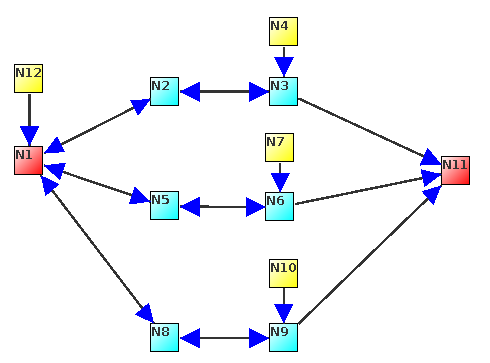
\includegraphics[height=7cm]{img/3_files.png}
        \caption{Modélisation d'une gare de péage avec trois files et deux
          moyens de payement}
        \label{figure:syphilis_3_2}
      \end{figure}

      Nous l'avons représenté comme suit:
      \begin{itemize}
        \item l'élément $N1$ représente toujours la route d'entrée;
        \item l'élément $N11$ représente la sortie;
        \item $N12$ permet de savoir quel moyen de payement va utiliser la
          voiture qui arrive dans $N1$ (s'il y en a) et va donc permettre de
          savoir vers quelle file la diriger;
        \item les éléments $N2$, $N5$ et $N8$ sont les files d'attente;
        \item les éléments $N3$, $N6$ et $N9$ sont les guichets de payement;
        \item les éléments $N4$, $N7$ et $N10$ permettent de savoir si une
          voiture dans la file a fini de payer: dans le cas de la file mixe
          carte bancaire/monnaie on considère qu'elle a fini de payer après un
          temps moyen $\frac 1 {\mu_m} = \frac{p_cb}{\mu_{cb}} +
          \frac{1-p_{cb}}{\mu_e}$.
      \end{itemize}

      \paragraph{Cas à deux files}
        En fixant $p_{cb} = 1$ on peut utiliser ce modèle pour gérer le cas
        $S=2$ files et un seul moyen de payement décrit dans la
        section~\ref{sec:peage_anal}.

        On remarque que l'analyse est conforme à l'expérience: un bouchon se
        crée si et seulement si $\lambda > 2\mu$.

      \paragraph{Critique du modèle}
        On remarque que (c'est logique!) on peut créer un bouchon seulement
        pour certains moyens de payement par exemple sur la file payement en
        espèce et payement quelconque mais pas payement par carte bancaire.
        Cependant notre modèle ne tient pas compte du type de payement qu'ont
        choisi les voitures au moment de se diriger vers une file: en effet si
        un tel bouchon se crée, toutes les voitures qui veulent payer par carte
        éviteront naturellement la file mixte mais notre modèle considérera
        toujours que $100 p_{cb}\%$ des voitures veulent payer par carte
        bancaire dans cette file.
\end{document}
